% Candidate source: src-2323f00197bbd8d5c8353a847fc0e7ccfc52169ca219272ee58990ae4b6ecba3
% Source PDF SHA-256: be2accb36a086126db90ee7c5a217e08e55429053a4167df1ad58bbfb213de46
% PDF page 1 (printed page 180), question 11.
% Redraw follows visible wave relations; schematic curve, not a scale claim.
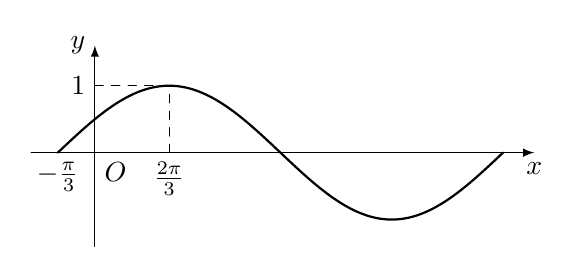
\begin{tikzpicture}[line cap=round,line join=round,>=latex,x=0.45cm,y=0.85cm]
  % Axes
  \draw[->] (-1.8,0) -- (12.4,0) node[below] {$x$};
  \draw[->] (0,-1.4) -- (0,1.6) node[left] {$y$};
  \node[below right] at (0,0) {$O$};

  % Function: f(x) = sin(0.5*x + pi/6), full period from -pi/3 to 11pi/3 landing on x-axis
  \draw[thick, smooth, domain={-3.1415926/3}:{11*3.1415926/3}, samples=100] plot (\x, {sin((0.5*\x + 3.1415926/6) r)});

  % Dashed projections for peak at (2pi/3, 1)
  \draw[dashed] ({2*3.1415926/3}, 0) -- ({2*3.1415926/3}, 1);
  \draw[dashed] (0, 1) -- ({2*3.1415926/3}, 1);

  % Ticks and labels
  \node[below] at ({-3.1415926/3}, 0) {$-\frac{\pi}{3}$};
  \node[below] at ({2*3.1415926/3}, 0) {$\frac{2\pi}{3}$};
  \node[left] at (0, 1) {$1$};
\end{tikzpicture}
